\chapter{Conclusions and discussion} \label{chap_conclusions}

This thesis culminates a multifaceted exploration into the convergence of \gls{ca} with
\gls{ns}. We have drawn upon the author's firsthand experience in designing Software
Architectures used rigorous theoretical research and created a practical and working
Software Artifact. The primary objective was to investigate the alignment between \gls{ca}
and \gls{ns}, by analyzing their principles and design elements through theory and
practice. This Chapter will summarize the findings into a research conclusion.

\section{Conclusion}

A noteworthy distinction between \gls{ns} and \gls{ca} lies in their foundational roots.
\gls{ns} is a product of computer science research built upon formal theories and
principles derived from rigorous scientific investigation. Although, throughout this
thesis, \gls{ns} is referred to as a development approach, it is a part of Computer
Science.

Stability and evolvability are concepts not directly referenced in the literature of
\gls{ca}, but very much aligns with the goal of \textcite[31]{mannaert_normalized_2016}.
The attentive reader surely observes the shared emphasis on modularity and the separation
of concerns. Both approaches attempt to achieve low coupling and high cohesion. In
addition, \gls{ca} add the dimensions of dependency management as an essential measure to
improve maintainability and manage modularity. 

A critical difference between \gls{ca} and \gls{ns} lies in their approach to handling
state. \gls{ca} does not explicitly address state management in its principles or design
elements. At the same time, \gls{ns} provides the principle of Separation of State,
ensuring that state changes within a Software System are stable and evolvable. This
principle can be crucial in developing scalable and high-performance systems, as it
isolates state changes from the rest of the system, reducing the impact of state-related
dependencies and side effects. This finding leads to the first conclusion of this thesis. 

\begin{enumerate}[leftmargin=*]
    \item The alignment between \gls{ca} and \gls{ns} is incomplete because \gls{ca} needs
    specific state management principles. As a result, \gls{ca} cannot fully ensure stable and
    evolvable software artifacts as defined by \gls{ns}.
\end{enumerate}

\section{Discussion}

Nevertheless, \gls{ns} and \gls{ca} can be effectively applied to enhance the stability and evolvability
of Software Systems. This synergetic relationship stems from the fact that NS contributes
a solid theoretical foundation for understanding and addressing the combinatorial effects
of system changes. At the same time, CA offers a robust, practical framework for
architectural design in software development.

By integrating the theoretical underpinnings of NS with the pragmatic principles of CA,
Software Architectures can harness both approaches' strengths to create stable software
systems and adaptable to changing requirements. In addition, the convergence of these
methodologies allows for a comprehensive understanding of the factors contributing to
reducing the complexity of the Software Architecture, enabling developers to make informed
design decisions prioritizing modularity, scalability, and extensibility, leading to the
last conclusion of this thesis.

The synergistic application of \gls{ns} and \gls{ca} can significantly improve software
systems' stability and evolvability. It leverages the advantages of both
approaches—combining \glspl{ns} rigorous theoretical basis with \glspl{ca} practical
guidelines for architectural design. This fusion of methodologies offers a powerful,
holistic approach to software development that addresses the challenges of system
complexity and fosters adaptability in an ever-evolving technological landscape.


\begin{enumerate}[resume, leftmargin=*]
    \item The alignment between \gls{ca} and \gls{ns} is incomplete because \gls{ca} needs
    specific state management principles. As a result, \gls{ca} cannot fully ensure stable and
    evolvable software artifacts as defined by \gls{ns}.
\end{enumerate}

\section{Reflections} \label{chap_reflection}

This section will dive into my enriching experiences and invaluable learnings acquired
while working on this research and thesis and is inspired by one of the master classes
about the \gls{ee} discipline. \gls{ee} encourages using grounded methodologies and
theories, like Five Way Framework, to comprehend the inner workings of an enterprise
\parencite[262]{dietz_enterprise_2020}. I will apply the so-called Five Way Framework to
reflect on this research. By incorporating the Five Way Framework into the section, I
aspire to coherently showcase my learnings and reflections, shedding light on my thought
processes, strategies, modeling techniques, working methodologies, and support mechanisms.

\begin{figure}[H]
    \centering
    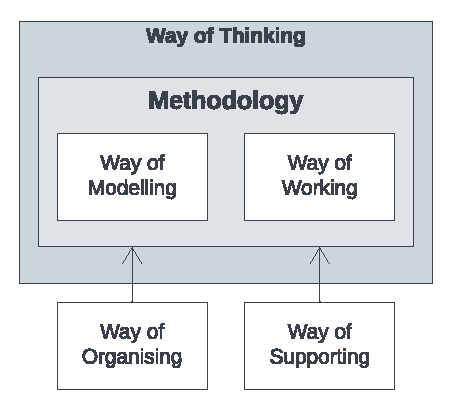
\includegraphics[width=0.5\textwidth]{figures/5ways.pdf}
    \caption[The Five Way Framework]{The Five Way Framework, inspired by \textcite{dietz_enterprise_2020}}
    \label{fig_5ways}
\end{figure}

\subsection{Way of Thinking}

Early in my career, I became obsessed with Software Quality and Maintainability. The
\gls{ns} theory shifted the obsession toward Stability and Evolvability. Gaining a
thorough understanding of the essential principles of this theory has boosted my
confidence in making informed decisions regarding all aspects of architecture, not just
limited to software.

As a Domain Architect, my job involved creating software products using the \gls{mdd}
paradigm. Initially, I was skeptical about this approach based on my early experiences.
The theory of \gls{ns} taught me to understand better the reasoning and characteristics of
code generation, on which I then realized that my skepticism was more about the process
caused as an effect on the implementation of the \gls{mdd}. The knowledge of \gls{ns}
helped me gain a clearer vision and helped me push the roadmap on the \gls{mdd} framework
in the right direction.

\subsection{Way of Modeling}

To explain the implementation concepts of the artifact, I looked into various modeling
languages. Archimate was the first option I considered. However, during one of the \gls{ee}
masterclasses, I learned the hard way that Archimate is not always the best choice for
communicating your models to a broad audience. I thought about using basic "boxes and
arrows" but decided to use the UML2 standard because it is a formal modeling language.

\subsection{Way of Working}

I very much enjoyed designing and creating the C\# artifacts. In hindsight, I enjoyed it
so much that I put in way too much effort than was needed. I was very curious about the
aspects of code generation, the effect of code generation on stable and evolvable
artifacts, and meta-circularity characteristics. I am confident I could have arrived at
the same conclusions presented in this thesis using a manually built Restful C\# artifact.
However, the insights I gained on the subjects of code expansion are of invaluable value
to me. Therefore, I am very pleased and satisfied that I took the effort to build the Code
Expander as a primary artifact. 

The \gls{ns} theorems are formulated very clearly and abstractly, making them also
applicable outside the software engineering field. During the masterclasses, we learned
about the application of \gls{ns} in the domains of Firewalls, Document management
systems, and Evolvable Business Processes. I also experienced benefits in structuring and
maintaining my Thesis document using \gls{vscode} and Latex by applying the principle of
\gls{soc} in managing the various chapters and sections. 

\subsection{Way of Organizing}

I should have been able to finish sooner. I was one of the first with a research topic and
started working on my artifact in the first month when starting this journey. The artifact
was as good as ready before the summer holidays of the first year. Unfortunately, I
postponed writing the thesis until a later moment. I want to think that next time I will
start sooner, but knowing myself, I need some pressure to perform the less fun tasks, like
writing this thesis.

The review process seemed difficult and sometimes even problematic for a couple of
reasons. Next time I will ensure having the proper tools and agree on procedures to
improve reviews from multiple proofreaders. Secondly, I noticed that having multiple
proofreaders sometimes steers in opposite directions. This sometimes affected my ability
to make decisions and negatively affected my confidence. Having a joined review document,
where all proofreaders can leave comments, will significantly improve this experience for
me and my proofreaders. Then there is the personal aspect of sometimes taking things too
personally, grounded in a lack of self-confidence. However, this experience improved my
self-confidence. 

\subsection{Way of Supporting}

At the beginning of my research, I received a thorough introduction to the \gls{ns}
Theories and the Prime Radiant tooling from an employer at NSX. This introduction was
extremely helpful in gaining a better understanding of the fundamentals of \gls{ns}. It
also inspired me to consider the Code Expansion as a primary artifact. 

For the writing of the Thesis, I decided to use Latex. I quickly discovered that Overleaf
was one of the most popular editors. Nevertheless, I continued my search since I rejected
the idea of relying on online tooling for writing my Thesis. At some point, I decided to
experiment with my favorite code editor \gls{vscode}, and with the help of a latex package
manager and some \gls{vscode} plugins, I was able to create a fully-fledged Latex Editor
in \gls{vscode}, being able to use all the other benefits that come with \gls{vscode}. In
my next project, I will likely use the \gls{vscode} Latex editor again.


% This thesis is the culmination of a multifaceted exploration into the convergence of
% \gls{ca} and \gls{ns}, drawing upon the author's firsthand experience in designing
% Software Architectures, rigorous theoretical research, and the development of a practical
% and working software artifact. The primary objective was to investigate the alignment
% between\gls{ca} and \gls{ns}. This was achieved by focussing the analysis on the
% principles and design elements of both approaches. This Chapter will summarize the
% findings into a research conclusion.

% A noteworthy distinction between \gls{ns} and \gls{ca} lies in their foundational roots.
% \gls{ns} is a product of computer science research, is built upon formal theories and
% principles that are derived from rigorous scientific investigation. Although \gls{ns} is
% mentioned as  
% can be considdered as a computer science it self. \gls{ca} can be considdered as a desing
% phylosophy, incorporating years of experience in a set of principles and best practices.
% Some of those principles also hav their foundation in science.

% both approaches share 
% shared emphasis on modularity, separation of concerns, and the reduction of dependencies
% between system components. Both approaches advocate for the creation of modular systems,
% with Clean Architecture focusing on the encapsulation of business logic within discrete
% use cases, and Normalized Systems emphasizing the separation of evolving and stable
% elements to enable incremental evolution. By adhering to these principles, developers can
% create software systems that are more maintainable, adaptable, and extensible, better
% equipped to cope with the ever-changing demands of the digital landscape.


%  The
% primary goal of NS is to create adaptable and maintainable software systems by addressing
% the combinatorial effects of system changes. NS principles are backed by mathematical
% models, enabling developers to systematically analyze and design software systems with a
% focus on modularity, scalability, and adaptability.


% The primary objective of this research has been to
% understand how integrating the principles of Clean Architecture and Normalized Systems can
% lead to the creation of adaptable, maintainable, and extensible software systems. Through
% a comprehensive examination of the underlying principles and design patterns, as well as
% practical implementation, this thesis has demonstrated that these two methodologies can
% indeed be harmonized to deliver enhanced benefits in software development, albeit with
% some considerations regarding state management.



% shedding light on the commonalities, differences, and synergies between these two
% approaches to software design. The primary objective of this research has been to
% understand how integrating the principles of Clean Architecture and Normalized Systems can
% lead to the creation of adaptable, maintainable, and extensible software systems. Through
% a detailed examination of the underlying principles and design patterns, this thesis has
% demonstrated that these two methodologies can indeed be harmonized to deliver enhanced
% benefits in software development, albeit with some considerations regarding state
% management.

% The convergence of Clean Architecture and Normalized Systems can be observed in their
% shared emphasis on modularity, separation of concerns, and the reduction of dependencies
% between system components. Both approaches advocate for the creation of modular systems,
% with Clean Architecture focusing on the encapsulation of business logic within discrete
% use cases, and Normalized Systems emphasizing the separation of evolving and stable
% elements to enable incremental evolution. By adhering to these principles, developers can
% create software systems that are more maintainable, adaptable, and extensible, better
% equipped to cope with the ever-changing demands of the digital landscape.

% A key difference between Clean Architecture and Normalized Systems lies in their approach
% to handling state. Clean Architecture does not explicitly address state management, while
% Normalized Systems provide the principle of Separation of State to ensure the proper
% handling of state changes within the system. This principle can be crucial in the
% development of scalable and high-performance systems, as it allows for the isolation of
% state changes from the rest of the system, reducing the impact of state-related
% dependencies and side effects.

% Incorporating the Separation of State principle from Normalized Systems into the Clean
% Architecture approach can enhance the overall software design by providing a more
% comprehensive solution to state management. By doing so, developers can create software
% systems that are not only modular and adaptable but also scalable and resilient. This
% holistic approach allows developers to capitalize on the strengths of each methodology
% while minimizing their limitations.

% Throughout this research, we have examined specific areas of alignment between Clean
% Architecture and Normalized Systems principles, such as the Interface Segregation
% Principle (ISP) and Action Version Transparency (AVT). We have established that these
% principles, while addressing different aspects of software design, can be combined to
% promote modularity and adaptability, resulting in a more robust software system. The
% Interface Segregation Principle encourages the creation of focused interfaces tailored to
% specific client needs, while Action Version Transparency allows for the coexistence of
% multiple versions of an action without affecting overall system behavior.

% In summary, the convergence of Clean Architecture and Normalized Systems offers a
% promising avenue for the development of software systems that are adaptable, maintainable,
% and extensible. By integrating the principles and practices of these two methodologies,
% including the Separation of State principle from Normalized Systems, developers can create
% robust software systems capable of addressing the complex and evolving needs of today's
% digital landscape. This thesis has provided a solid foundation for understanding the
% synergies between Clean Architecture and Normalized Systems, paving the way for further
% research and practical application of these approaches in real-world software development
% projects.

% As the field of software engineering continues to evolve, it is crucial for developers and
% researchers alike to explore new avenues for collaboration and integration between
% different methodologies. By embracing the convergence of Clean Architecture and Normalized
% Systems, including the proper handling of state, we can further advance the state of the
% art in software development, fostering the creation of innovative, resilient, and
% adaptable software systems that stand the test of time.

% \begin{enumerate}
%     \color{red}

%     \item \textbf{Literature Review}
%     \begin{itemize}
%         \item Ca offers structure, principles and guidelines on how to build something. On top
%         of that, NST also offers guidelines in order to apply actual changes.
%         \\gls{ca} has a strong emphasis on testability of code. Coupling is an important
%         aspect on this.
%         \item \gls{srp} differs fundamentally from \gls{soc} in definition, although in
%         the artifact not that much (further explain). Komt vooral door verschillende
%         definities in granulariteit.
%     \end{itemize}
    
%     \item \textbf{Architectural Desing}
%     \begin{itemize}
%         \item 
%     \end{itemize}

%     \item \textbf{Artifact Development}
%     \begin{itemize}
%         \item 
%     \end{itemize}
%     \begin{enumerate}[label*={\arabic*.}]
        
%         \item \textbf{The Code Generator and Clean Architecture Expander}
%         \begin{itemize}
%             \item 
%         \end{itemize}
        
%         \item \textbf{Expanded Clean Architecture artifact}
%         \begin{itemize}
%             \item 
%         \end{itemize}
        
%     \end{enumerate}
    
%     \item \textbf{Convergence Analysis:}
%     \begin{itemize}
%         \item 
%     \end{itemize}
%     \begin{enumerate}[label*={\arabic*.}]
        
%         \item An analysis per principle of \gls{ca}, compared with each of the principles
%         of \gls{ns}, indicating each level of convergence per principle
        
%         \item An analysis per element of \gls{ca}, compared with each of the elements of
%         \gls{ns}, indicating each level of convergence per principle
    
%     \end{enumerate}
% \end{enumerate}
